\documentclass{article}
\usepackage{amsmath}   % for mathematical equations
\usepackage{graphicx}  % for including graphs and images
\usepackage{float}     % to force figure placement
\usepackage{caption}   % for figure captions
\usepackage{siunitx}   % for units formatting
\usepackage{hyperref}  % for links

\title{Lab Report 1: Lab 1 - 3}
\author{Enrique Rivera Jr \\ Marcus}
\date{\today}

\begin{document}
\maketitle

\begin{center}
\section*{Lab 1: Basic Measurements and Oscilloscope Use}
\end{center}

\section{Introduction}
This lab introduces basic electronic measurement techniques using a multimeter and oscilloscope. 
The objective is to measure DC and AC voltages, understand the concept of output impedance, and 
analyze waveforms using a function generator. By constructing simple circuits, we will learn 
how to measure voltage, current, and impedance, and observe the behavior of waveforms under 
different conditions.

\section{Methods / Notes}
    \subsection{Breadboard Layout and Measurement}
    Using a multimeter in buzzer mode, we first determined the internal connections of a 
    breadboard. The multimeter's buzzing feature was used to identify connected holes.

    \begin{figure}[H]
        \centering
        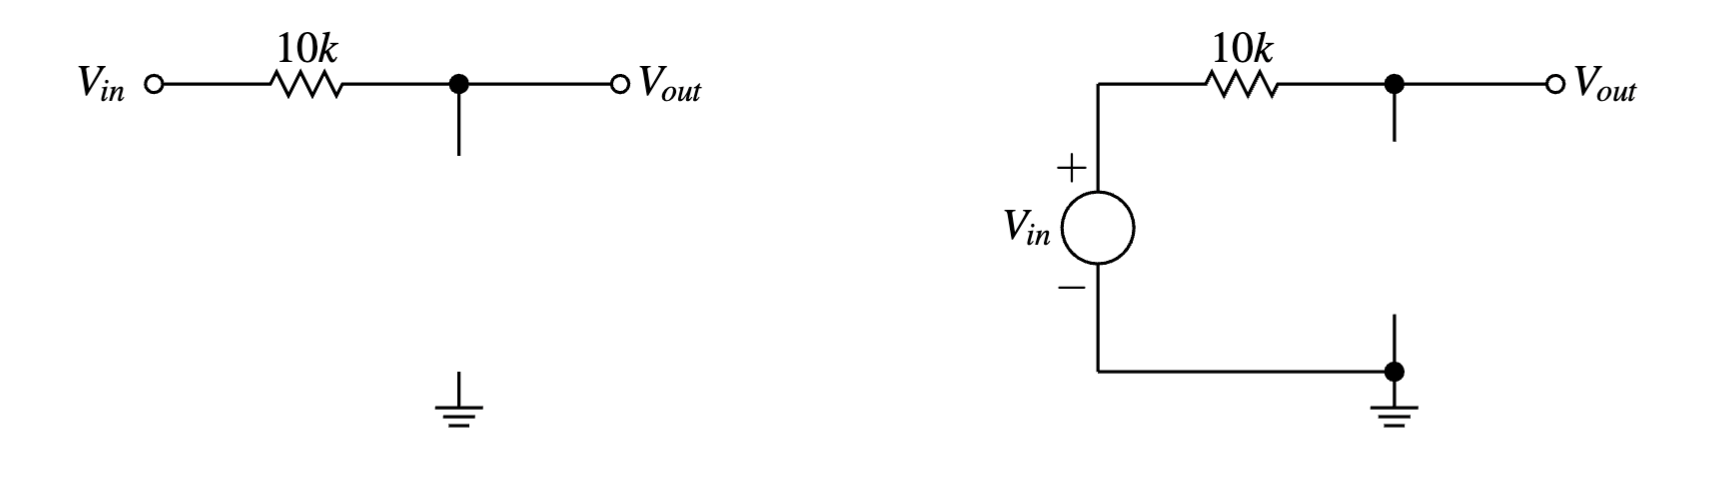
\includegraphics[width=0.8\textwidth]{img/other/Open_Circuit.png} % Replace with actual image path
        \caption{Open Circuit}
        \label{fig:opencircuit}
    \end{figure}

    \begin{figure}[H]
        \centering
        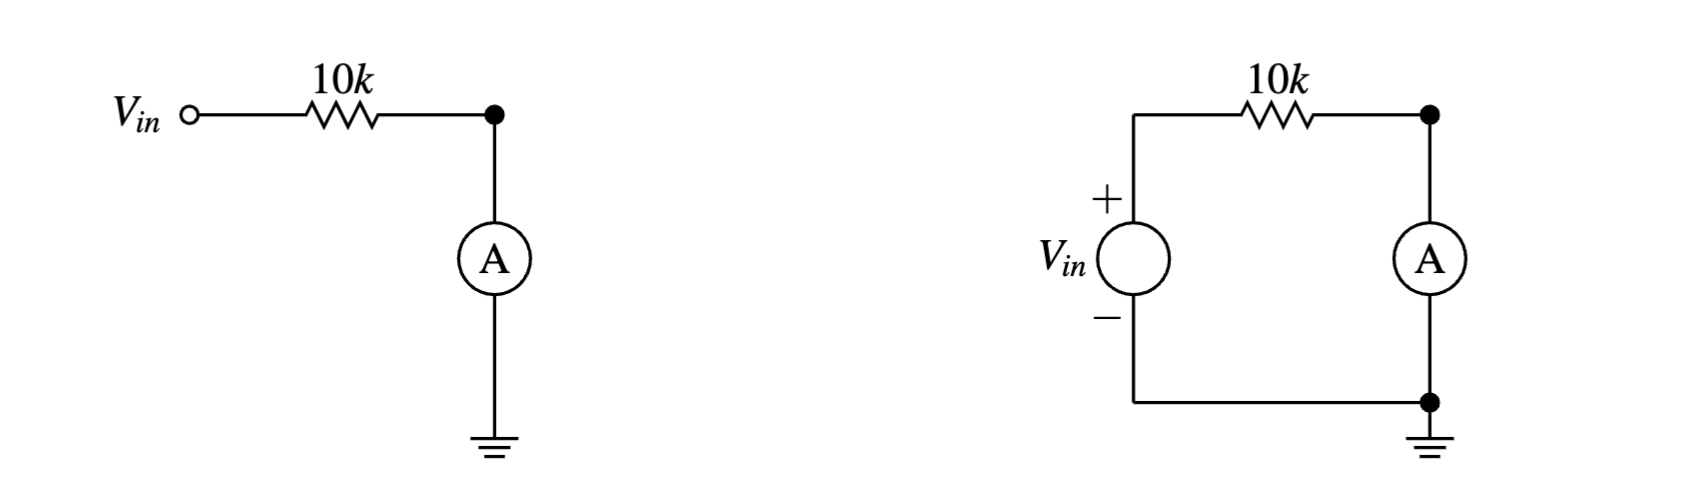
\includegraphics[width=0.8\textwidth]{img/other/Close_Circuit.png} % Replace with actual image path
        \caption{Closed Circuit}
        \label{fig:closedcircuit}
    \end{figure}

\subsubsection{Open and Closed Circuit Measurements}
The open circuit was constructed as shown in Figure \ref{fig:opencircuit}. The DC power supply 
was set to 5V, and the voltage was measured across the open circuit using the multimeter. Next, a c
losed circuit was constructed, and the current was measured using the ammeter function.


The output impedance $Z_{out}$ was calculated using the formula:
\[
Z_{out} = \frac{V_{\text{open}}}{I_{\text{closed}}}
\]

\subsubsection{Voltage Divider}
A voltage divider was constructed using two resistors of equal value (10k$\Omega$ each), and the output voltage was measured across the second resistor. The theoretical voltage was calculated using the voltage divider formula:
\[
V_{out} = V_{in} \times \frac{R_2}{R_1 + R_2}
\]

Both the measured and calculated voltages were recorded.

\subsubsection{Function Generator and Oscilloscope}
The output of a function generator was connected to an oscilloscope. 
A 1kHz sine wave with 2V peak-to-peak was generated. The waveform was observed and 
recorded on the oscilloscope screen. The effect of adding a 50$\Omega$ terminator was 
noted, and both the terminated and unterminated waveforms were sketched and compared.

\subsection{Results}
    \subsubsection{(1) Breadboard Layout}
    The following diagram shows the internal connections of the breadboard. The multimeter was used 
    to map out which holes were connected.

    \begin{figure}[H]
        \centering
        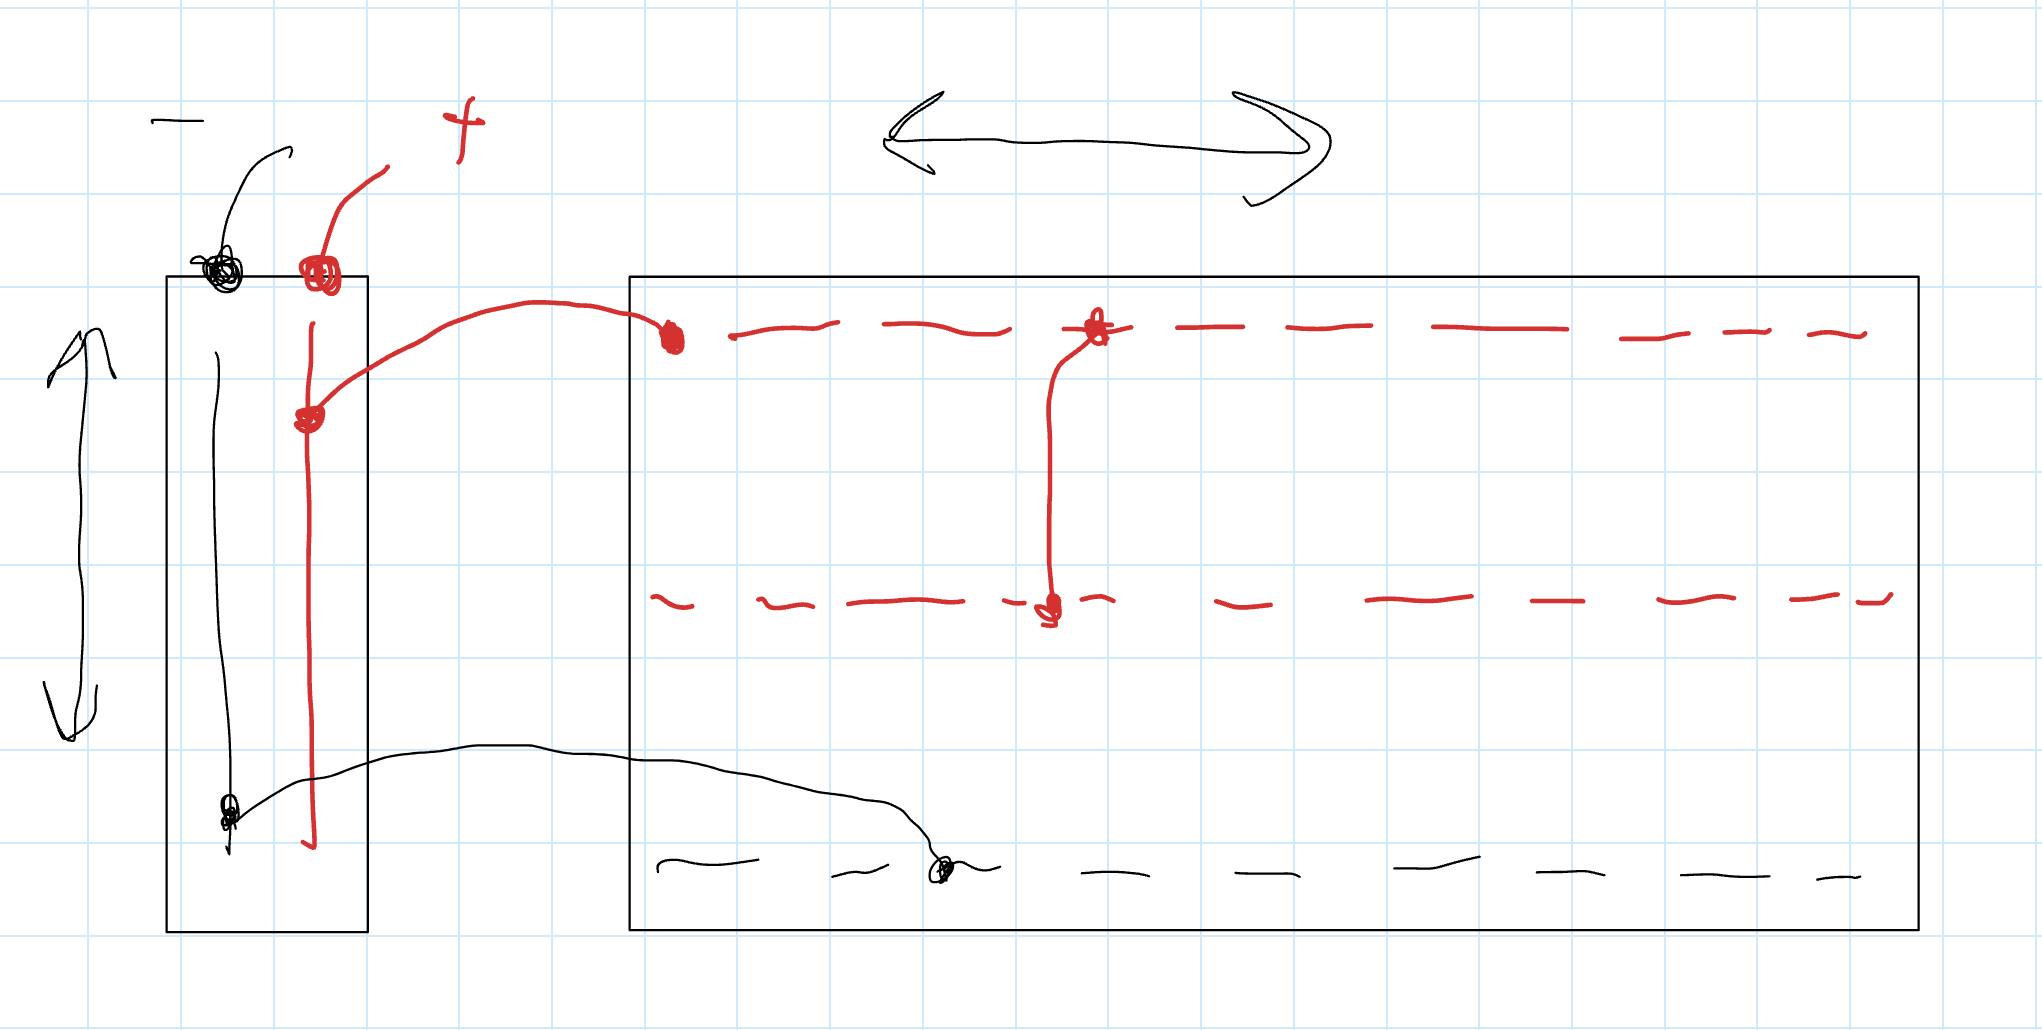
\includegraphics[width=0.8\textwidth]{img/Lab1_1.png} % Replace with actual image path
        \caption{How a breadboard`s internal connections are laid out.}
        \label{fig:breadboard_layout}
    \end{figure}


    \subsubsection{(2c) Open and Closed Circuit Measurements}
    The measured open circuit voltage was \SI{5}{V} and the closed circuit current was \SI{0.5}{A}. Using these values, the output impedance was calculated to be:
    \[
    Z_{out} = \frac{5 \text{V}}{0.5 \text{A}} = 10 \, \Omega
    \]

    \subsubsection{(3) Voltage Divider Results}
    The measured output voltage for the voltage divider was \SI{2.5}{V}, matching the theoretical calculation.

    \begin{table}[H]
    \centering
    \caption{Voltage Divider Results}
    \begin{tabular}{|c|c|c|}
    \hline
    $V_{in}$ (V) & $V_{out}$ (Measured) (V) & $V_{out}$ (Calculated) (V) \\ \hline
    5            & 2.5                      & 2.5                        \\ \hline
    \end{tabular}
    \end{table}

    \subsubsection{(4) Voltage Divider Cases}
    The following cases were considered for the voltage divider. When R2 $\gg$ R1, the output voltage is 
    approximately equal to the input voltage. When R2 $\ll$ R1, the output voltage is approximately zero.

    \begin{figure}[H]
        \centering
        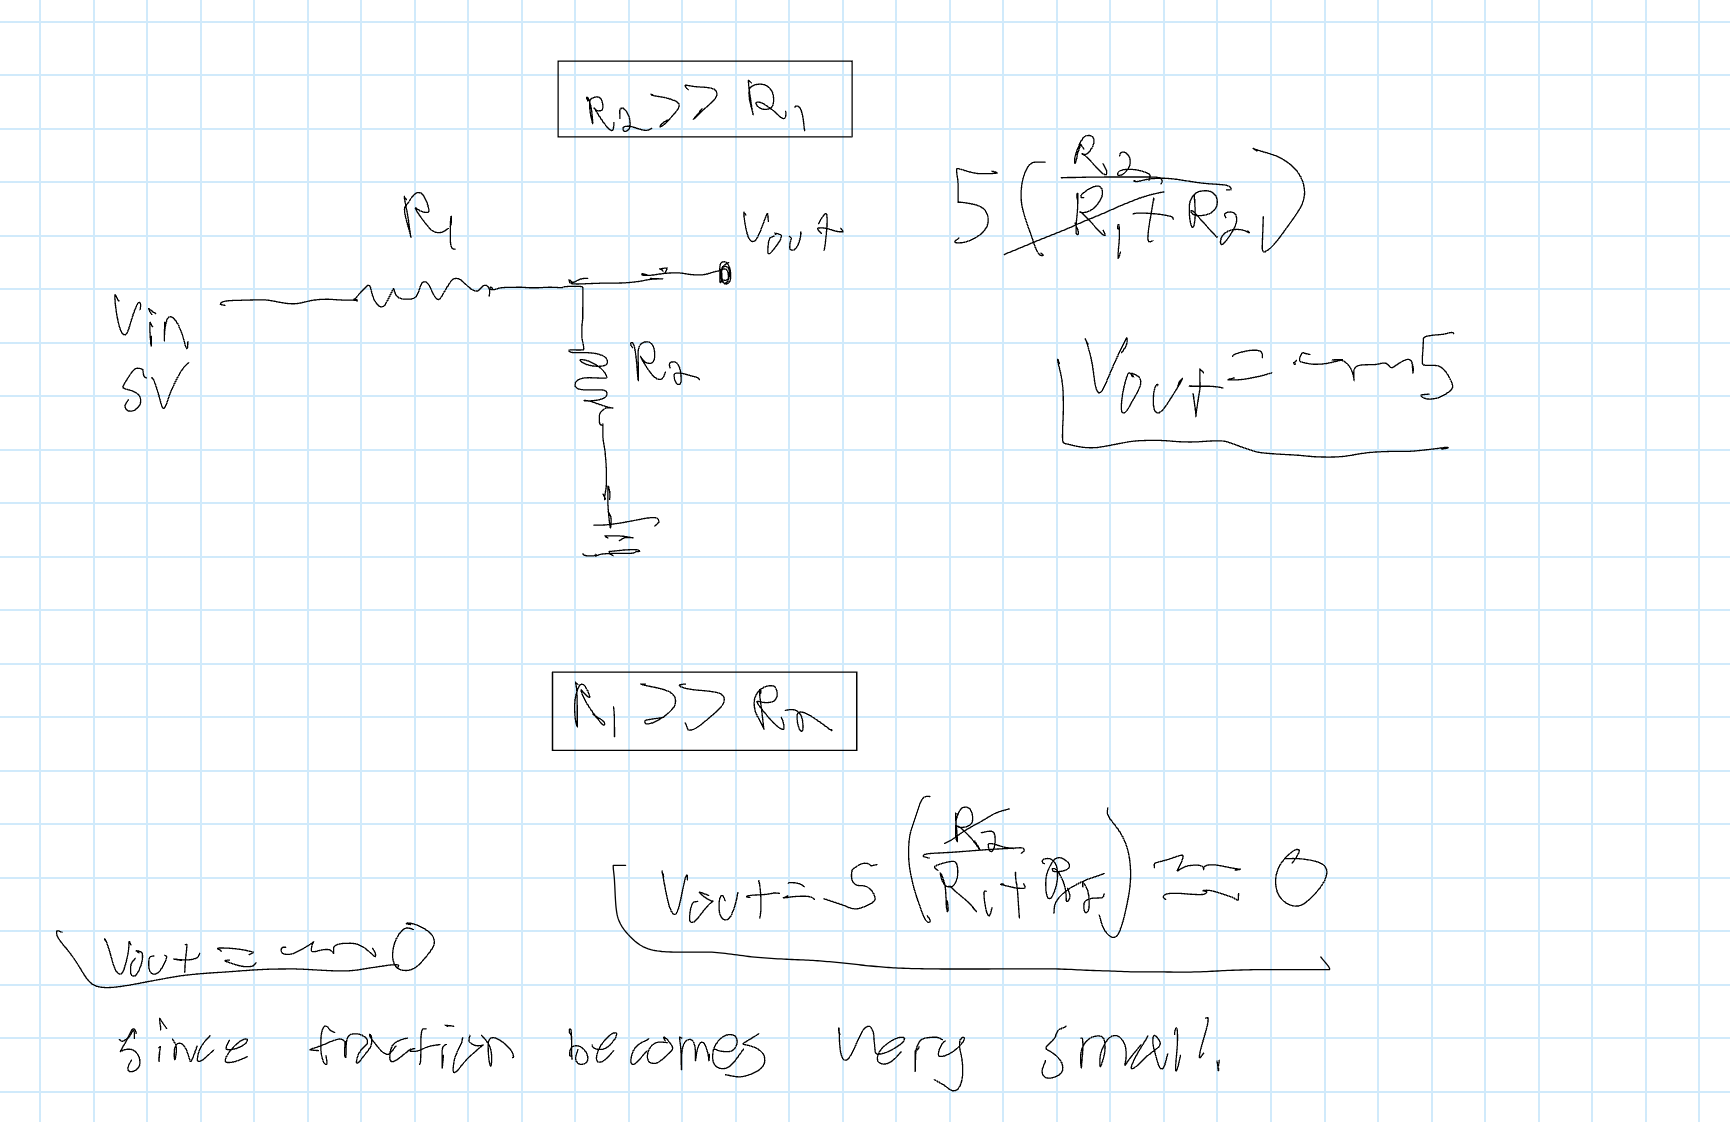
\includegraphics[width=0.9\textwidth]{img/Lab1_4.png}  % Replace with actual path
        \caption{Voltage Divider Cases}
        \label{fig:voltage_divider_cases}
    \end{figure}

    \subsubsection{(5) Function Generator and Oscilloscope}
    The following waveforms were observed using the oscilloscope for the function generator output.

    \begin{figure}[H]
        \centering
        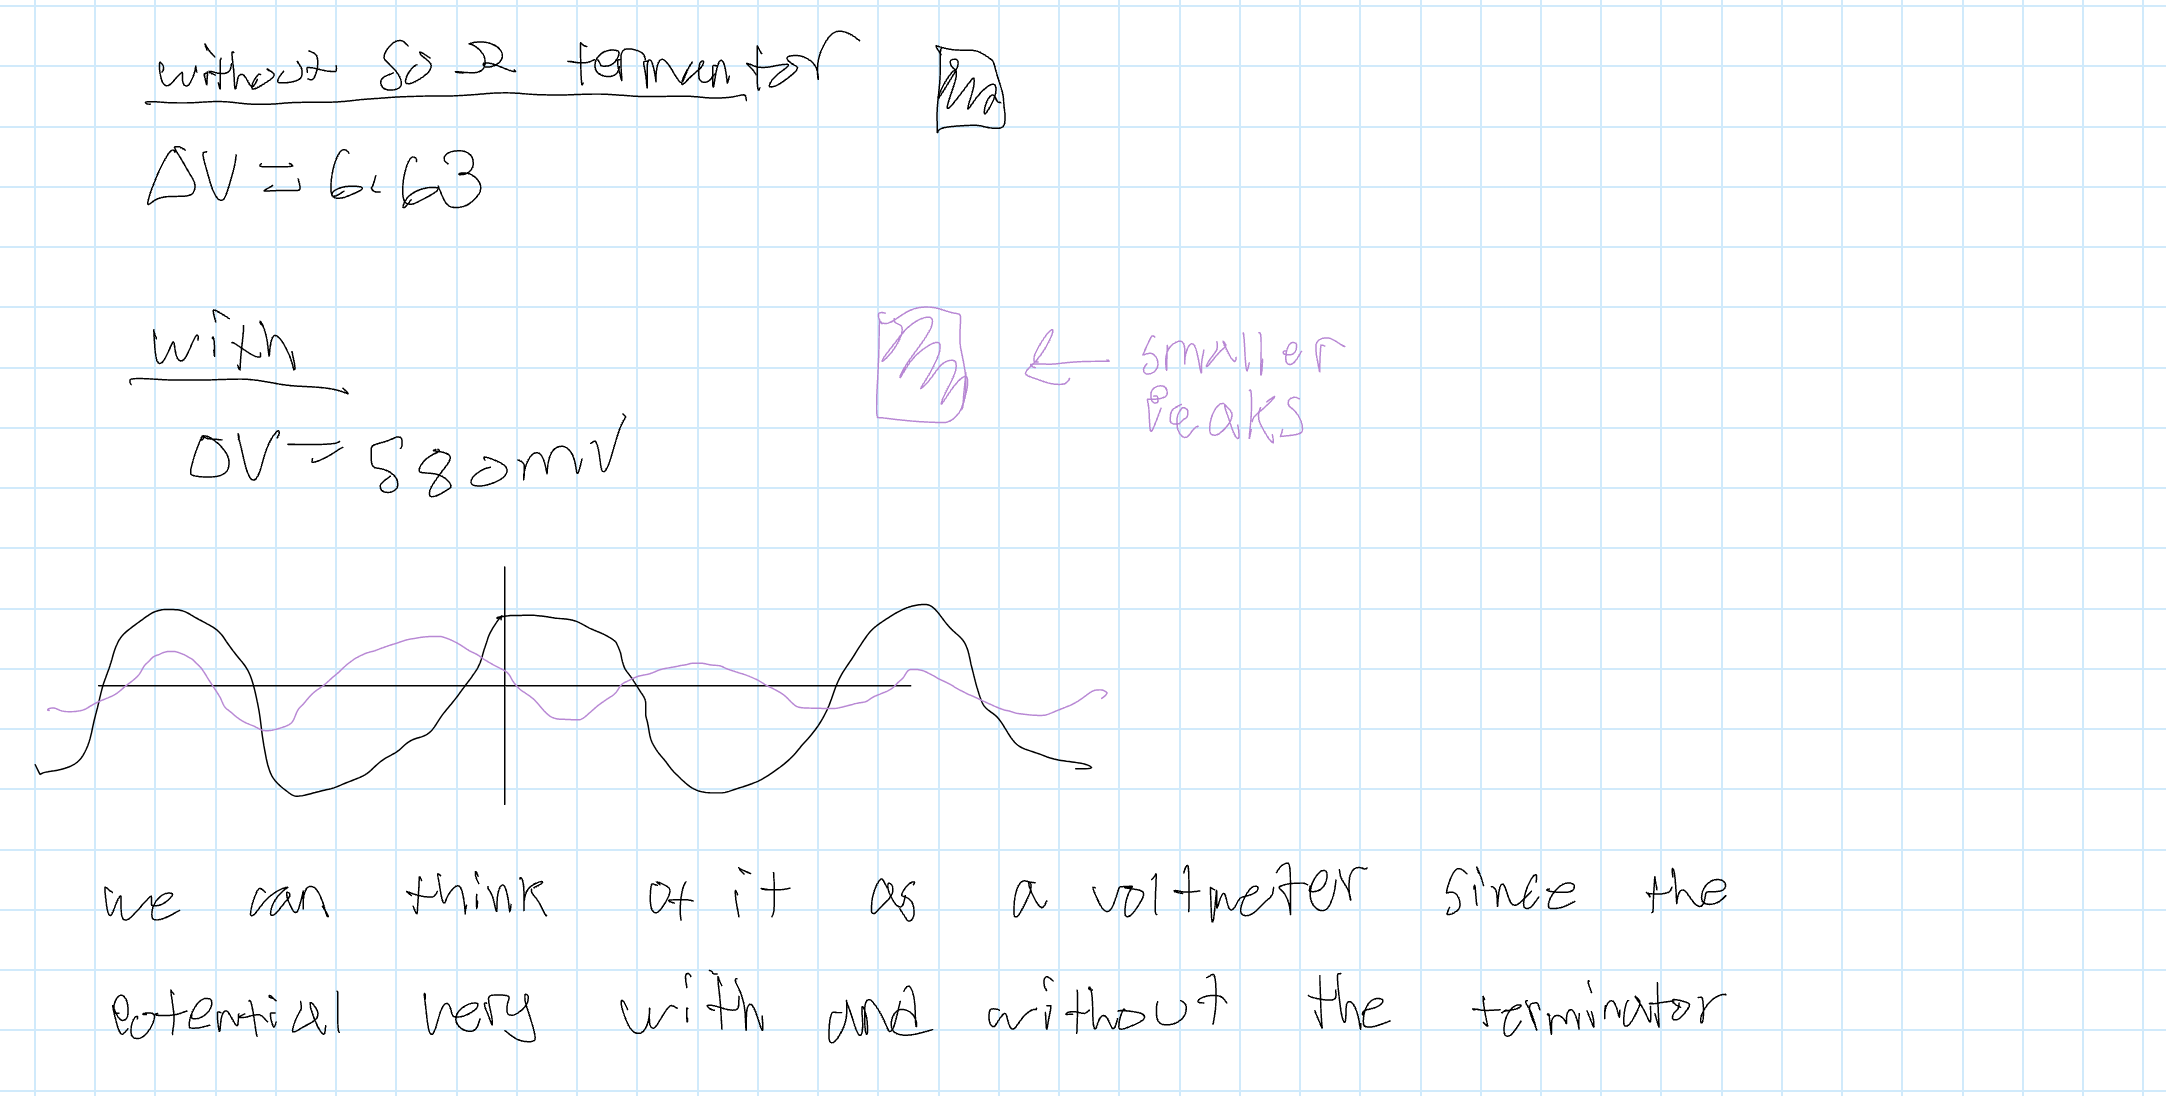
\includegraphics[width=0.9\textwidth]{img/Lab1_5.png}  % Replace with actual path
        \caption{Waveform with terminator connected and disconnected.}
        \label{fig:terminated_waveform}
    \end{figure}

    \subsubsection{(6) Trigger Effect}
    The trigger effect was observed by adjusting the trigger level and observing the waveform on the oscilloscope. 
    
    \begin{figure}[H]
        \centering
        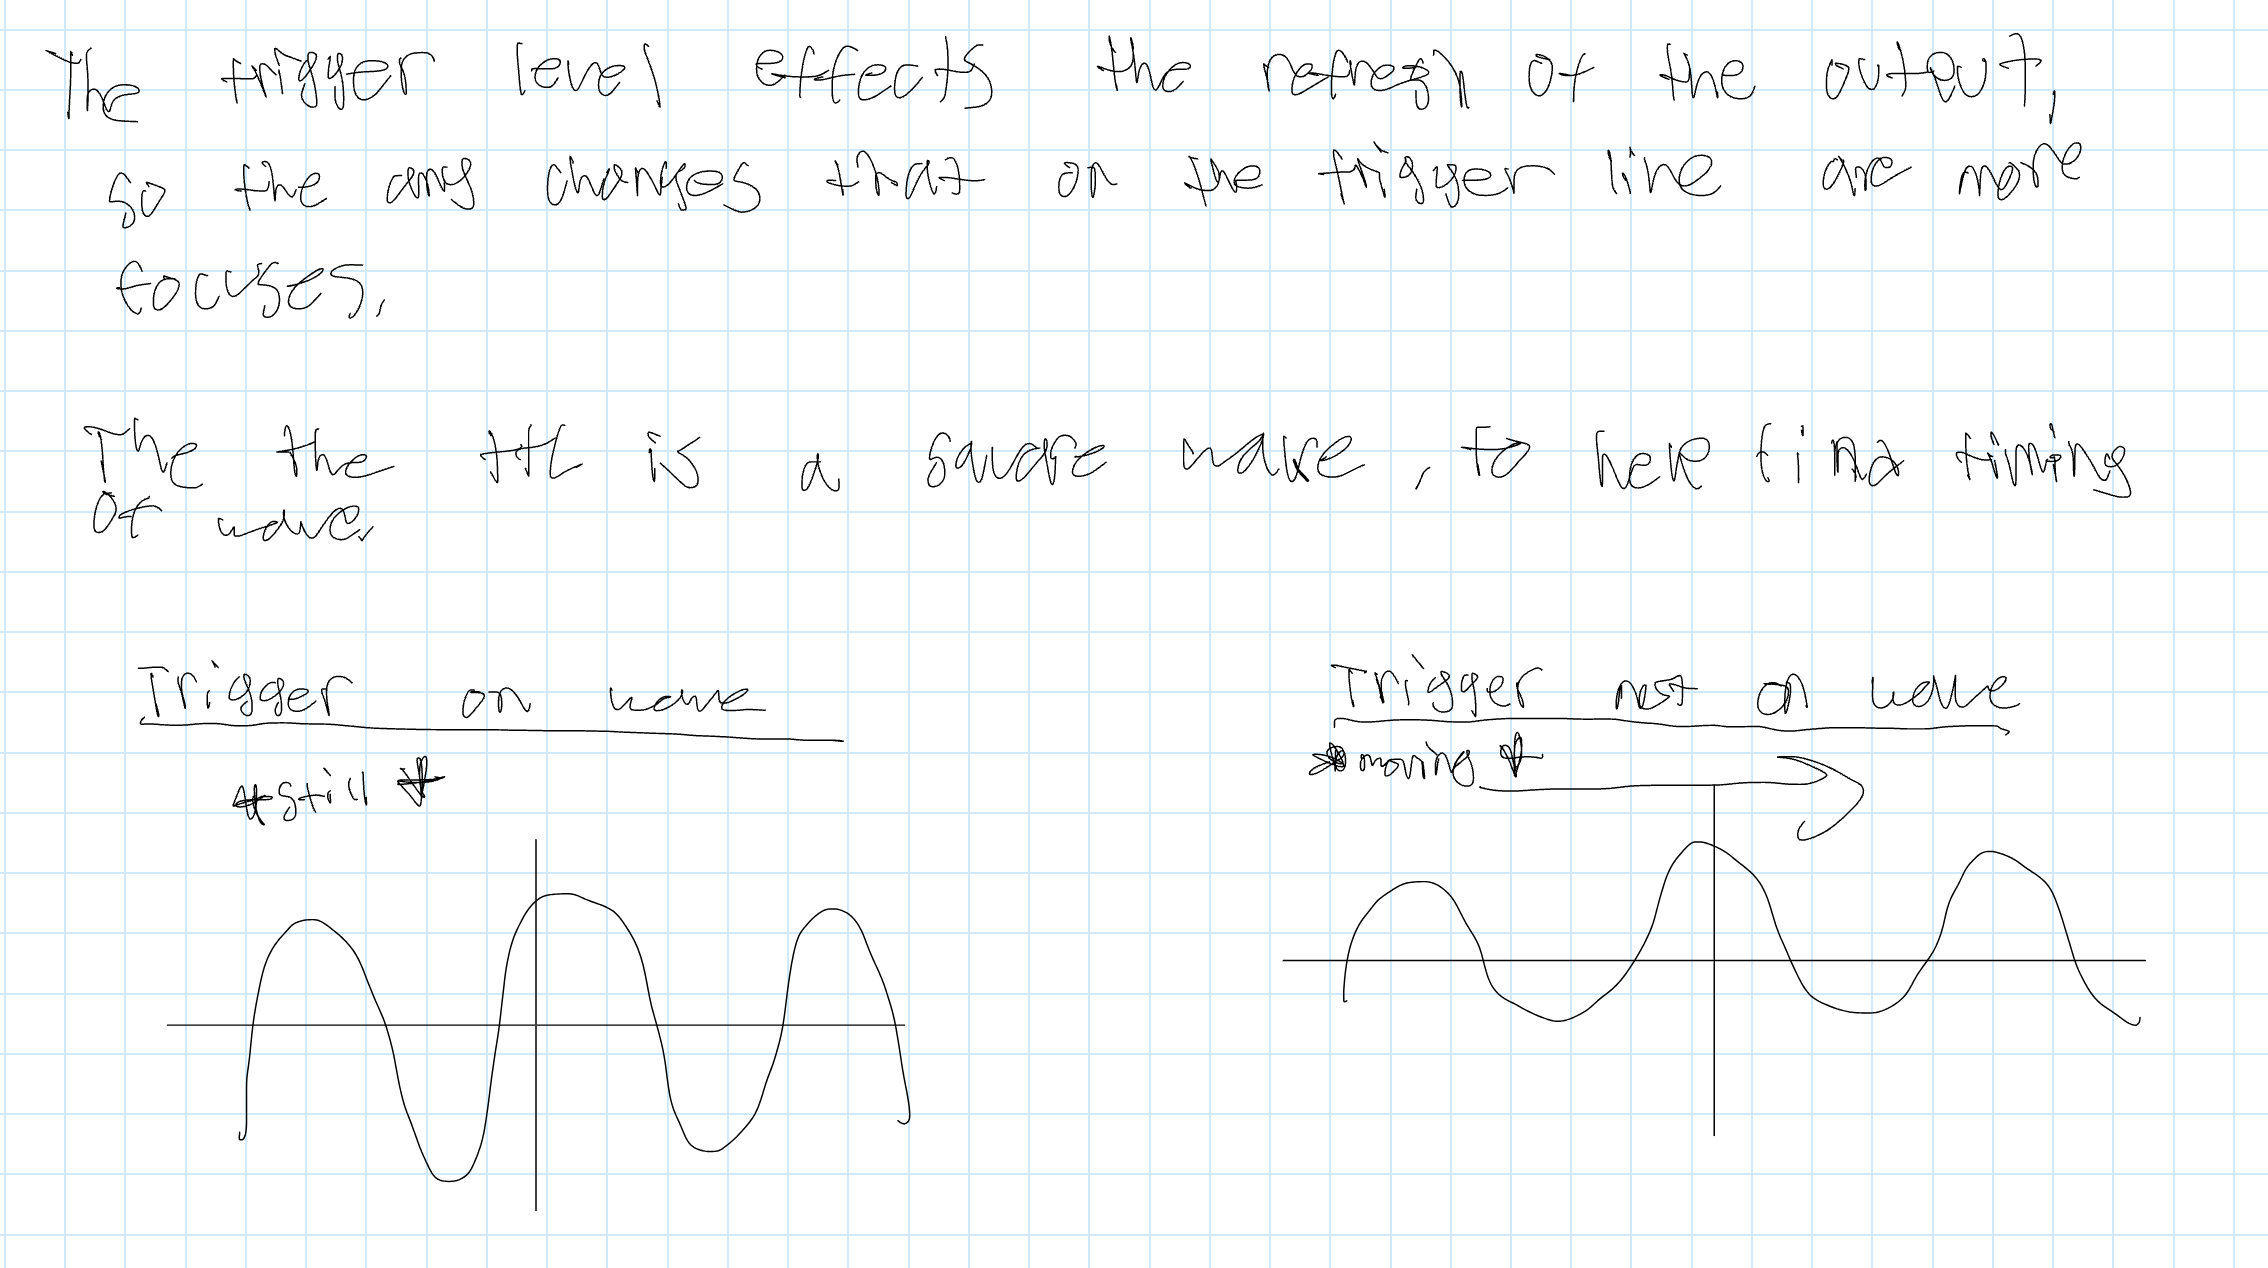
\includegraphics[width=0.9\textwidth]{img/Lab1_6.png}  
        \caption{Waveform with Trigger Level adjusted.}
        \label{fig:trigger_waveform}
    \end{figure}

    \subsubsection{(7) DC Offset Effect}
    The DC offset effect was observed by adjusting the DC offset and observing the waveform on the oscilloscope. 
    
    \begin{figure}[H]
        \centering
        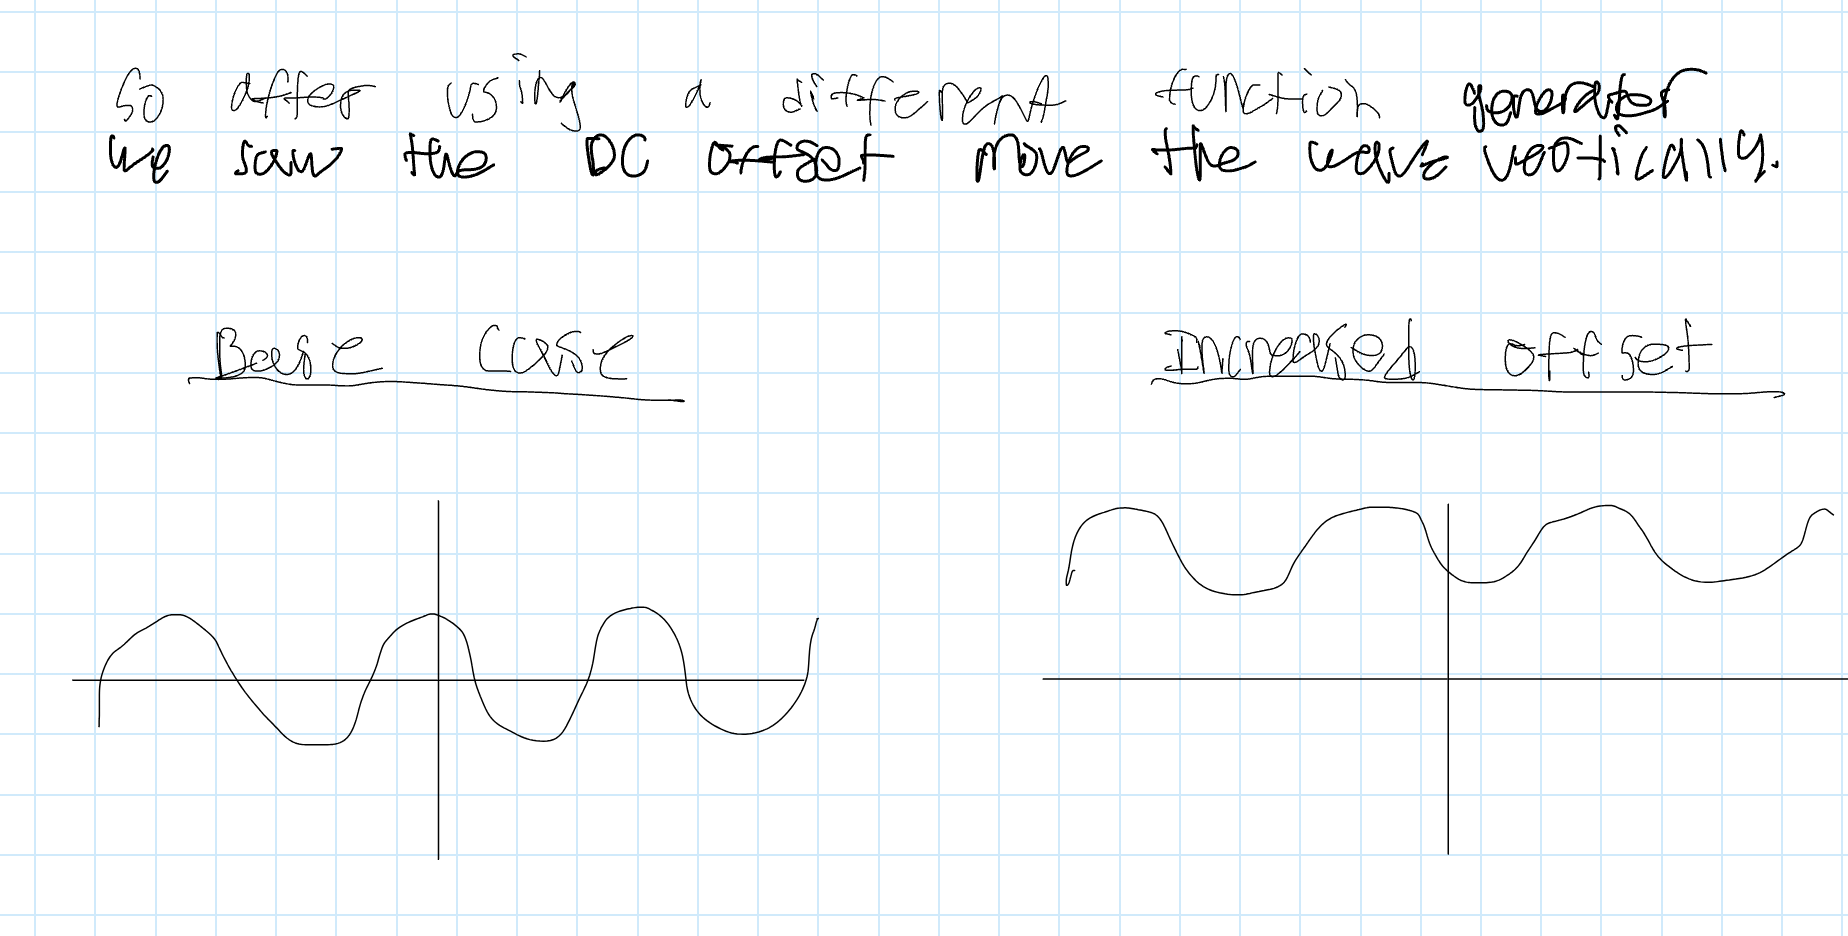
\includegraphics[width=0.9\textwidth]{img/Lab1_7.png}  
        \caption{Waveform with terminator connected and disconnected.}
        \label{fig:terminated_waveform}
    \end{figure}

    \subsubsection{(8) Voltage Divider Formula}
    The DC offset effect was observed by adjusting the DC offset and observing the waveform on the oscilloscope. 
    
    \begin{figure}[H]
        \centering
        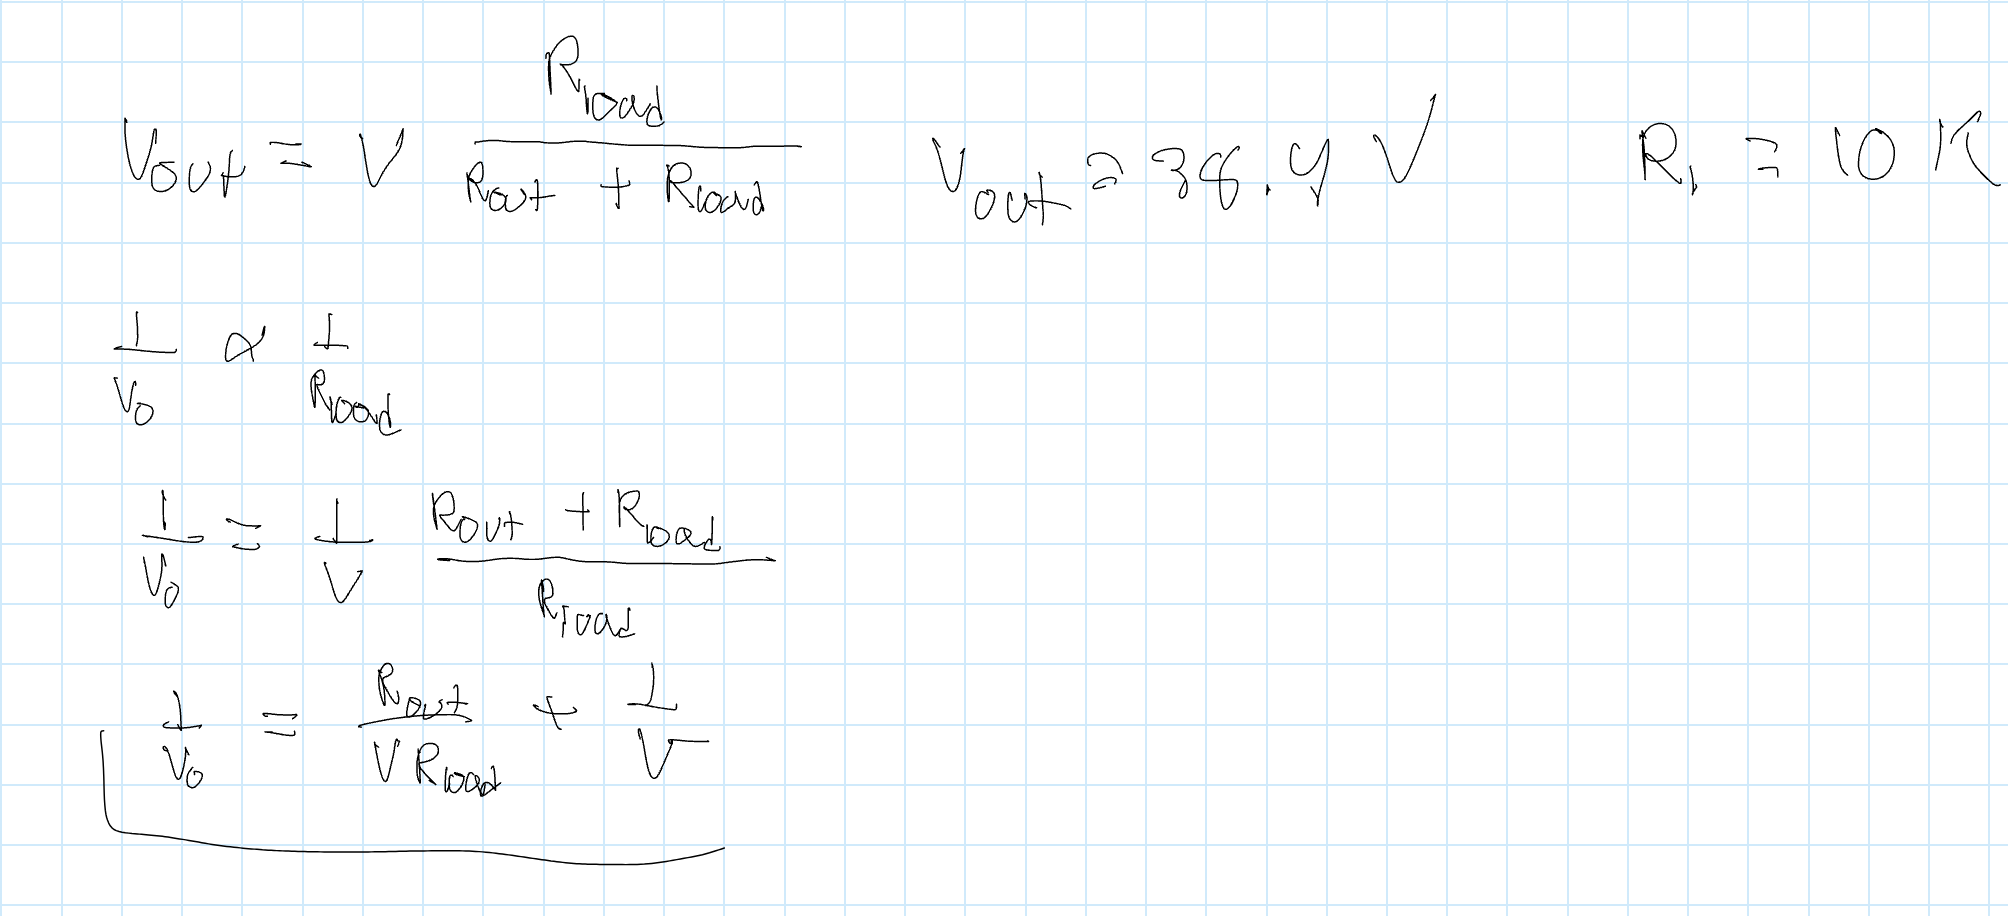
\includegraphics[width=0.9\textwidth]{img/Lab1_8.png}  
        \caption{Derived Voltage Formula.}
        \label{fig:Derived Voltage Formula}
    \end{figure}

    \begin{figure}[H]
        \centering
        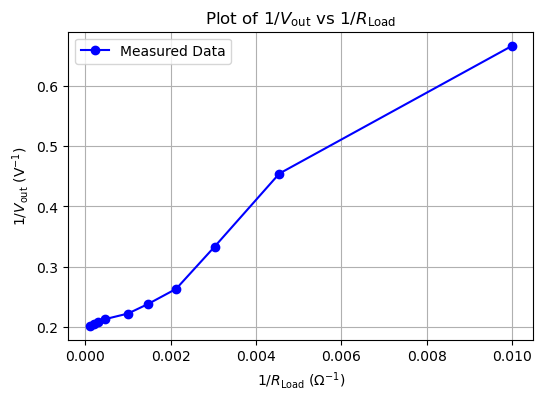
\includegraphics[width=0.9\textwidth]{img/Lab1_8a.png}  
        \caption{Graph of $V_{out}$ vs. $R_{load}$}
        \label{fig:Derived Voltage Formula Graphs}
    \end{figure}

    \subsubsection{(9) RMS amplitude }
    \begin{figure}[H]
        \centering
        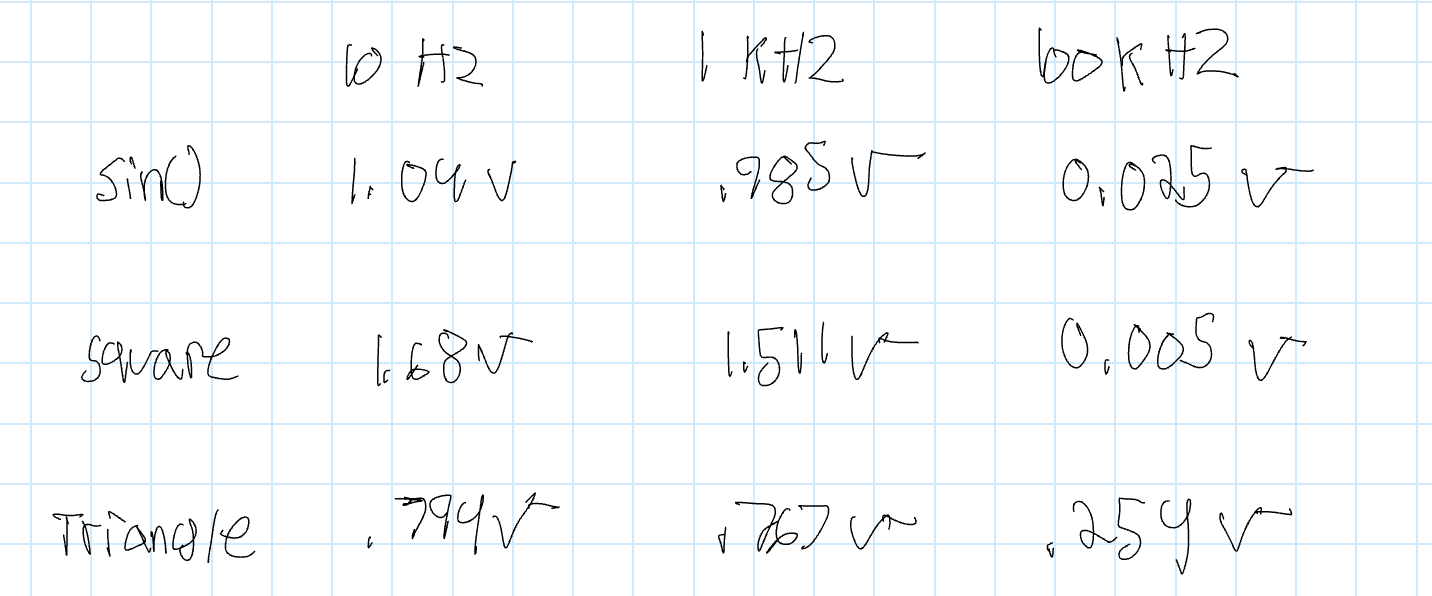
\includegraphics[width=0.9\textwidth]{img/Lab1_9.png}  
        \caption{Graph of $V_{out}$ vs. $R_{load}$}
        \label{fig:RMS amplitude}
    \end{figure}

    \subsubsection{(10) Measured rise (or fall) Time }
    The rise time was measured to be 0.35 ns.

\begin{center}
    \section*{Lab 2}
\end{center}


\begin{center}
    \section*{Lab 3}
    \end{center}

\end{document}
